\documentclass[10pt,a4paper,twocolumn]{article}
\usepackage[utf8]{inputenc}
\usepackage[portuguese]{babel}
\usepackage[T1]{fontenc}
\usepackage{apacite}
\usepackage{amsmath}
\usepackage{amsfonts}
\usepackage{amssymb}
\usepackage{tikz}
\usepackage{graphicx}
\usepackage{refstyle}
\usepackage{hyperref}
\usepackage{float}
\usepackage{natbib}
\usepackage{url}
\usepackage{listings}
\usepackage[export]{adjustbox}
\usepackage{xcolor}
\definecolor{ds}{rgb}{0.87,0.89,0.92}
\lstdefinestyle{mystyle}{
    backgroundcolor=\color{ds},   
    commentstyle=\color{red},
    keywordstyle=\color{magenta},
    numberstyle=\tiny\color{gray},
    stringstyle=\color{purple},
    basicstyle=\ttfamily\footnotesize,
    breakatwhitespace=false,       
    breaklines=true,                 
    captionpos=b,                    
    keepspaces=true,                 
    numbers=left,                    
    numbersep=5pt,                  
    showspaces=false,                
    showstringspaces=false,
    showtabs=false,                  
    tabsize=2
}
\lstset{style=mystyle}
\usetikzlibrary{calc,patterns,angles,quotes,babel}
\usepackage[left=2cm,right=2cm,top=2cm,bottom=2cm]{geometry}
\author{Sony Gonzaga de Melo Neto - 119110023}
\title{Análise do Experimento do Pêndulo Simples na Célula de Carga \\
 \large Universidade Federal de Campina Grande \\
  Disciplina: Instrumentação Científica \\
  Professor Adriano de A. Batista}
\hypersetup{colorlinks=true, linkcolor=blue}
\begin{document}
\maketitle
\section{INTRODUÇÃO}
\par Este relatório descreverá o processo experimental e a análise de dados de um pêndulo simples obtidos utilizando uma célula de carga, tendo como objetivo a extração da frequência de oscilação do pêndulo.
\par A célula de carga é um aparato eletrônico que tem como principal função a medição da intensidade de uma força aplicada sobre ele. No geral, as células de carga são compostas por um material que se deforma microscopicamente ao ser nele aplicada uma força. Essa deformação modifica as propriedades estruturais do material e comuta na alteração de sua resistência elétrica. A mudança na resistência provoca variação numa corrente atuando sobre ele, que pode ser interpretada como sinais num osciloscópio e traduzida como informações da força originalmente aplicada.
\par Esse instrumento, por possuir bastante exatidão nas medidas, é amplamente utilizado principalmente na fabricação de balanças de precisão.
\section{DESCRIÇÃO DO EXPERIMENTO}
\par No experimento em questão, uma extremidade de uma corda foi acoplada à uma célula de carga e na outra colocou-se uma massa para executar-se oscilações como as de um pêndulo simples. 
\par O pêndulo foi deixado para balançar por um período de 20 segundos, enquanto os sinais, em Volts, foram registrados no computador num arquivo .csv (Comma-separated values), para cada ponto correspondente no domínio do tempo.
\section{O PÊNDULO SIMPLES}
\begin{figure}[H]
\begin{center}
\begin{tikzpicture}
 % save length of g-vector and theta to macros
    \pgfmathsetmacro{\Gvec}{1.5}
    \pgfmathsetmacro{\myAngle}{30}
    % calculate lengths of vector components
    \pgfmathsetmacro{\Gcos}{\Gvec*cos(\myAngle)}
    \pgfmathsetmacro{\Gsin}{\Gvec*sin(\myAngle)}

    \coordinate (centro) at (0,0);
    \draw [dashed,gray,-] (centro) -- ++ (0,-3.5) node (mary) [black,below]{$$};
    \draw [blue,-stealth] (centro) -- ++ (0,-1.5) 
    
    node[midway,left] {$F$};
    \draw[thick] (centro) -- ++(270+\myAngle:3) coordinate (bob)
    node[midway,right] {$l$};;
    \pic [draw, ->, "$\theta$", angle eccentricity=1.5] {angle = mary--centro--bob};
    \draw [blue,-stealth] (bob) -- ($(bob)!\Gcos cm!(centro)$)
      node[midway,right] {$T$};
    \draw [-stealth] (bob) -- ($(bob)!-\Gcos cm!(centro)$)
      coordinate (gcos)
      node[midway,above right] {$g\cos\theta$};
    \draw [-stealth] (bob) -- ($(bob)!\Gsin cm!90:(centro)$)
      coordinate (gsin)
      node[midway,above left] {$g\sin\theta$};
    \draw [-stealth] (bob) -- ++(0,-\Gvec)
      coordinate (g)
      node[near end,left] {$g$};
    \pic [draw, ->, "$\theta$", angle eccentricity=1.5] {angle = g--bob--gcos};
    \filldraw [fill=black!40,draw=black] (bob) circle[radius=0.1]
    node[right] {$m$};
\end{tikzpicture}
\end{center}
\caption{Diagrama de um Pêndulo Simples}
\label{fig:pendulo}
\end{figure}
\par O pêndulo simples é um sistema físico de um movimento harmônico, com sua trajetória obedecendo um arco de circuferência. Por conta disso, o ângulo $\theta$ varia com o tempo, fazendo sua aceleração tangencial $g\sin\theta$ também ser função do tempo, portanto, o movimento descrito é oscilatório.
\par A força de aceleração $g\cos\theta$ se equilibra com $T$, portanto, a única força atuante no sistema é $g\sin\theta$, com o único grau de liberdade $\theta$. A equação de movimento, então, é:
\begin{equation}
\ddot{\theta}+\frac{g}{l}\sin\theta=0.
\end{equation}
\par Para ângulos muito pequenos, $sin\theta\approx\theta$, e a solução da equação será:
\begin{equation}
\theta(t)=\theta_0\cos(\sqrt{\frac{g}{l}}t).
\end{equation}
\par O termo $\sqrt{\frac{g}{l}}$ é denominado de frequência angular do pêndulo, denotada por $\omega$. Como $\omega=2\pi f$, sendo $f$ a frequência de oscilação, 
\begin{equation}
\label{eqn:freq}
f=\frac{1}{2\pi}\sqrt{\frac{g}{l}}.
\end{equation}
\section{ANÁLISE DOS DADOS}
\par Os dados registrados são exibidos por meio de um programa em Python, que utiliza a biblioteca matplotlib para esse propósito. São dois conjuntos de dados, um cru, formado pelas medições diretas da célula de carga:
\begin{figure}[H]
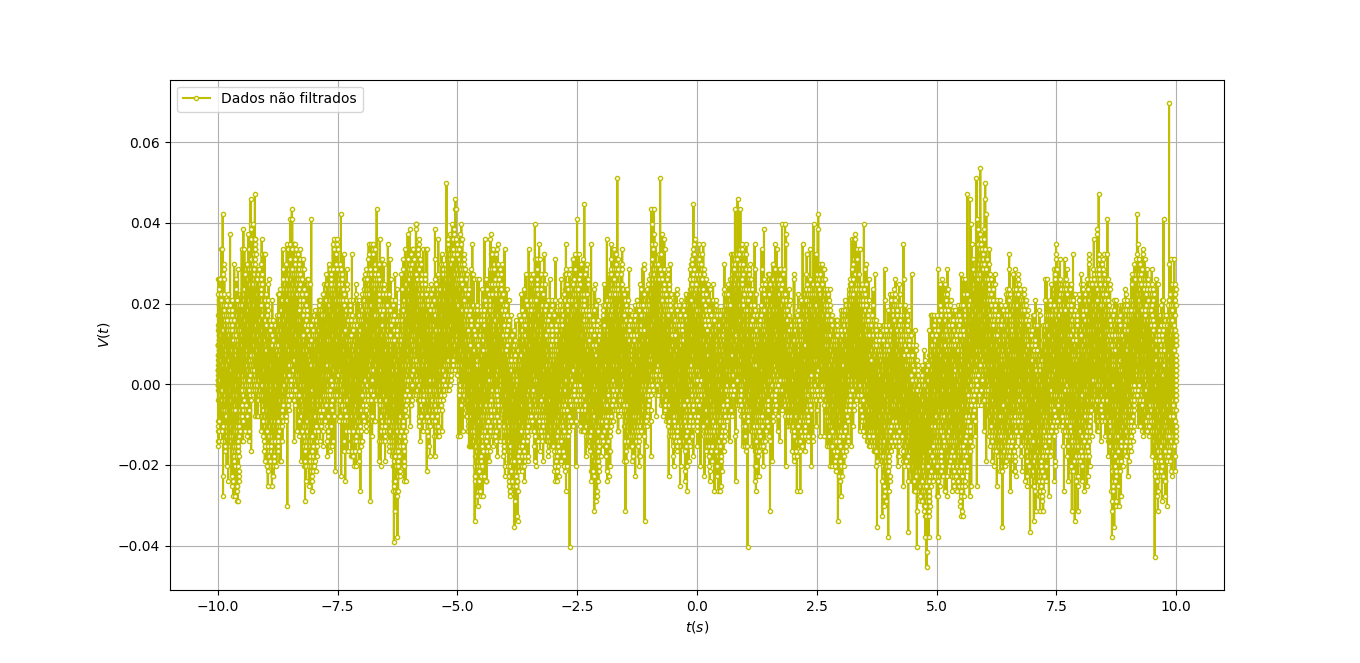
\includegraphics[width=0.5\textwidth, left]{NãoFiltrados}
\caption{Dados não filtrados}
\label{fig:naofiltrados}
\end{figure}
e outro com um filtro aplicado:
\begin{figure}[H]
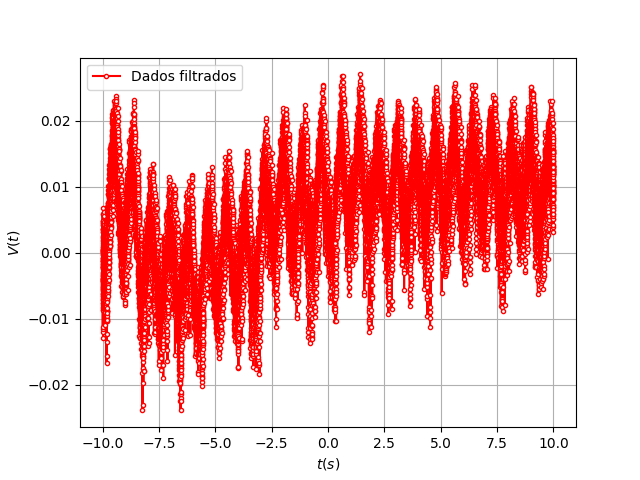
\includegraphics[width=0.5\textwidth, left]{Filtrados}
\caption{Dados filtrados}
\end{figure}
\par Para os dados não filtrados da Figura \ref{fig:naofiltrados}, utiliza-se um Filtro de Média Móvel, utilizando a biblioteca Pandas. O Filtro de Média Móvel calcula a média entre $n$ sinais e a transforma em um novo sinal. Fazendo isso com todos os pontos, os ruídos serão atenuados. Caso $n$ seja muito pequeno, pouco ruído sumirá, mas, caso $n$ seja muito grande, as características originais do gráfico serão perdidas, como sua propriedade oscilatória. 
\par O Filtro de Média Móvel segue a seguinte equação:
\begin{equation}
y[t]=\frac{1}{n}\sum_{k=0}^{n-1}x[t-k].
\end{equation}
\par Os dados, ao passar pelo filtro com $n=649$, ficarão: 
\begin{figure}[H]
\includegraphics[width=0.5\textwidth, left]{Filtradosmm}
\caption{Dados filtrados com Filtro de Média Móvel}
\label{fig:filtradosmm}
\end{figure}
É importante observar que a frequência das oscilações obtidas nos sinais da célula de carga é o dobro da frequência de oscilação do pêndulo. Isso pode ser explicado ao verificar que na Figura \ref{fig:pendulo}, a força $F$ medida pela célula de carga é uma componente da tensão $T$: $F=T\cos\theta$. Como $T$ também é componente da força peso, $T=mg\cos\theta$, há a implicação $F=mg(\cos\theta)^2$. Utilizando a identidade trigonométrica $(\cos\theta)^2=\frac{1}{2}(1+\cos2\theta)$, conclui-se que $F=\frac{1}{2}mg(1+\cos2\theta)$, que tem frequência duas vezes a do pêndulo.
\par A obtenção da frequência de oscilação é feita de duas maneiras, por medição direta e por Transfomada de Fourier.
\subsection{MEDIÇÃO DIRETA}
Para a medição direta da frequência, cria-se um programa que traça retas entre as posições no tempo entre os máximos e mínimos do gráfico com a biblioteca Scipy.
\par Nesse caso, o programa identificará os mínimos como os máximos do gráfico espelhado no eixo do horizontal, subtraído da diferença entre seus valores de maior e menor intensidade, para manter os pontos mínimos sempre abaixo dos máximos. Apesar da amplitude ser diferente, a frequência independe desta.
\par A partir desses pontos, mede-se a diferença entre um máximo e um mínimo consecutivos para todos os períodos, excluindo os primeiros e últimos máximos e mínimos (o programa pode identificar os primeiros e últimos pontos como um máximo ou um mínimo relativo). A média aritimética dessas diferenças dará metade do período médio. A frequência obtida por esse experimento, portanto, será função desse período médio.
Para achar o melhor valor de $n$, faz-se um algoritmo que encontre o maior valor da frequência em função do $n$. Esta função terá um único pico máximo, portanto, executa-se o algoritmo com os valores da frequência num range razoável que contenha o melhor valor de $n$. O melhor valor encontrado é $n=649$, já usado anteriormente.
\par Os gráficos correspondentes à cada conjunto de dados, com cada frequência do pêndulo encontrada, seguem:
\begin{figure}[H]
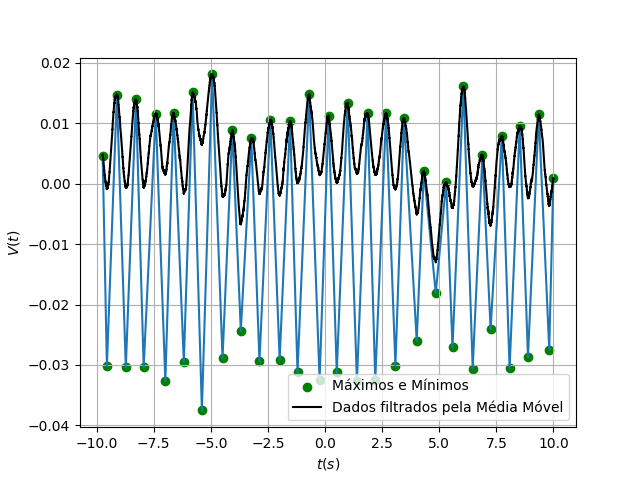
\includegraphics[width=0.5\textwidth, left]{MDFiltradosMM}
\caption{Medida Direta com os Dados Filtrados pela Média Móvel. $f=0,602119 Hz$ \centering}
\label{fig:mdfiltradosmm}
\end{figure}
\begin{figure}[H]
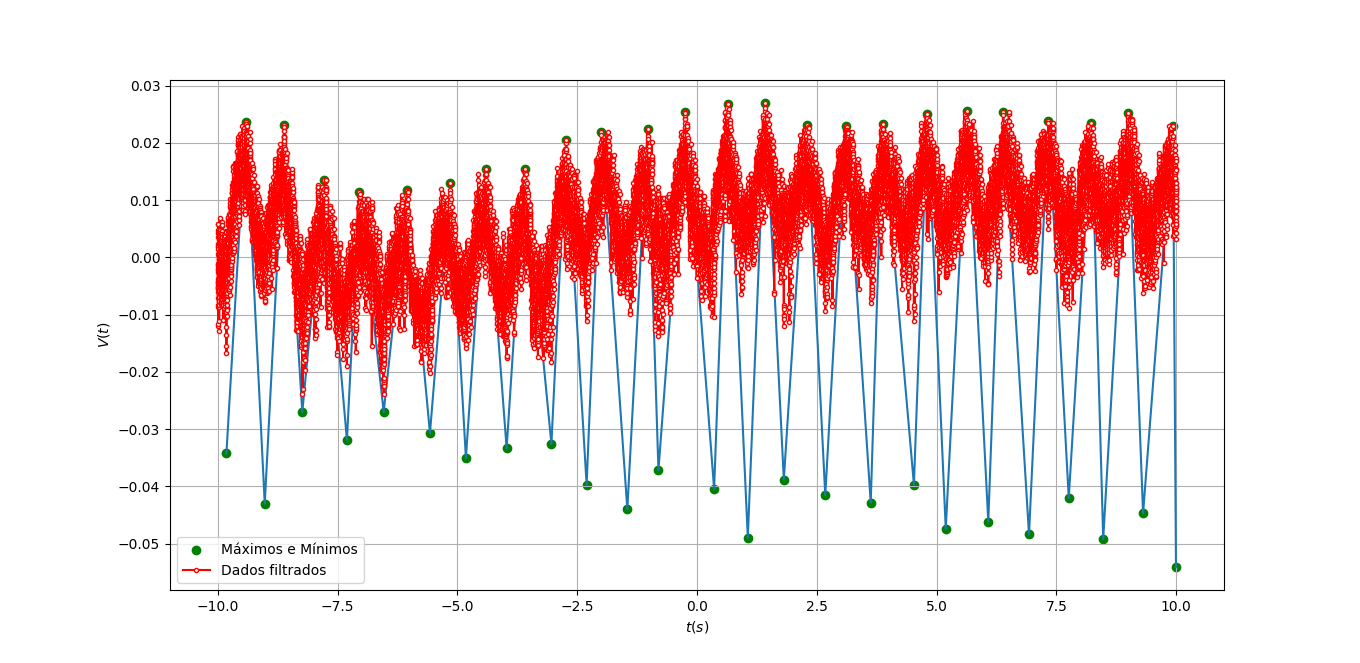
\includegraphics[width=0.5\textwidth, left]{MDFiltrados}
\caption{Medida Direta com os Dados Filtrados.
 $f=0,612355 Hz$ \centering}
\label{fig:mdfiltrados}
\end{figure}
\subsection{TRANSFOMADA DE FOURIER}
\par Para a obtenção da frequência de oscilação utilizando a Transformada de Fourier, utiliza-se um programa escrito com base na biblioteca Scipy que plote o gráfico da T.F. de um gráfico de oscilação no domínio das frequências.
\par O gráfico da T.F. apresentará vários pontos discretos que correspondem às frequências que compõem o gráfico de oscilações e seus respectivos pesos. A frequência mais distinta diferente de zero, a do pêndulo, será a mais proeminente, enquanto as outras são resultantes dos ruídos, podendo ser descartadas.  
\par Para os dados não filtrados, é mais precisa a aplicação da T.F. direta, sem passar pelo filtro. Seguem, portanto, as T.F. com as frequências do pêndulo encontradas:
\begin{figure}[H]
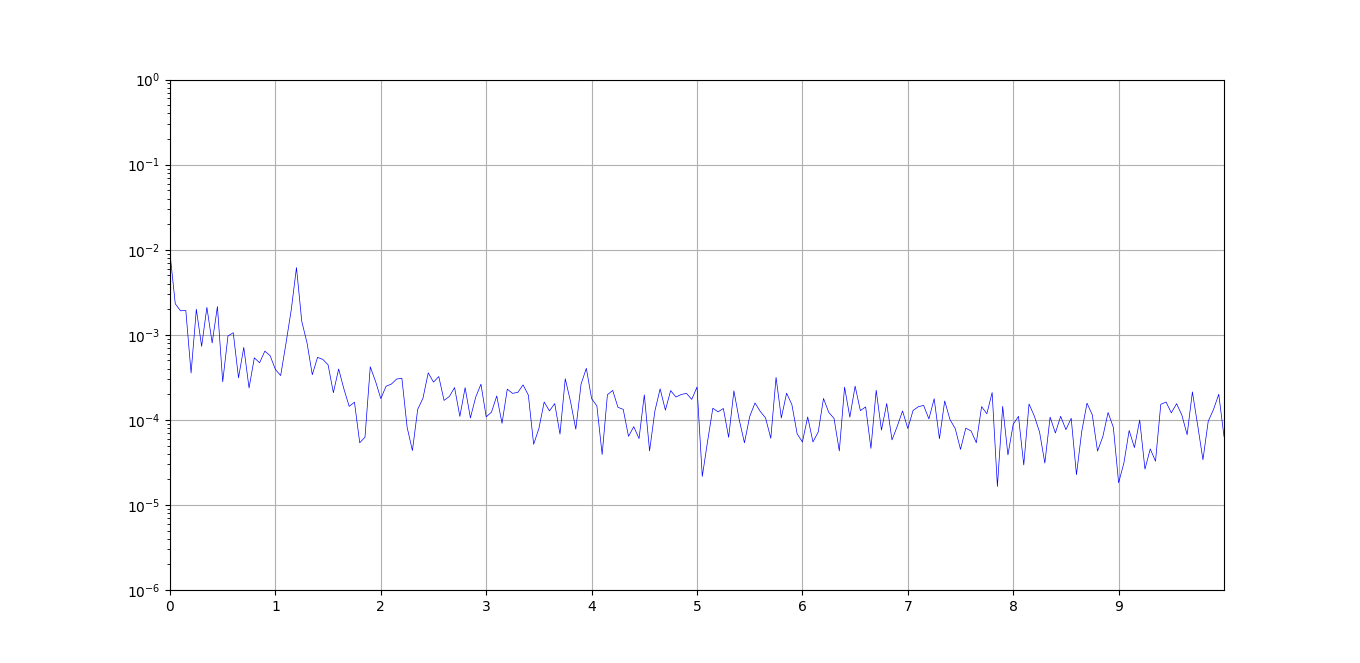
\includegraphics[width=0.5\textwidth, left]{TFNãoFiltrados}
\caption{Transformada de Fourier com os Dados Não Filtrados.
 $f=0,60003 Hz$ \centering}
\label{fig:tfnaofiltrados}
\end{figure}
\begin{figure}[H]
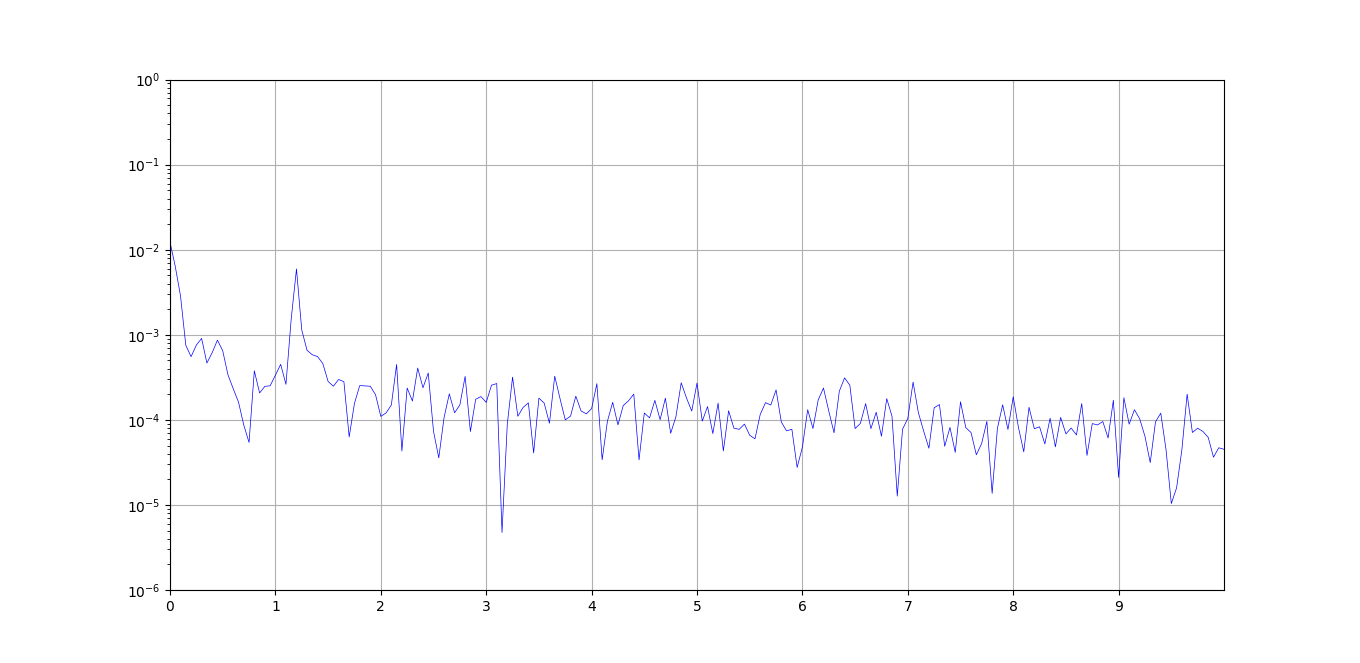
\includegraphics[width=0.5\textwidth, left]{TFFiltrados}
\caption{Transformada de Fourier com os Dados Filtrados.
 $f=0,60001 Hz$ \centering}
\label{fig:tffiltrados}
\end{figure}
\section{CONCLUSÃO}
\par Da análise por medição direta, conclui-se que a frequência de oscilação do pêndulo é $f_1=(0,6072\pm0,0051) Hz$, enquanto a encontrada pela análise das Transformadas de Fourier é $f_2=(0,60002\pm0,00001) Hz$.
\par Portanto, vê-se que a Transformada de Fourier é um método bem mais eficiente e preciso para a análise dos dados (nesse caso, estacionários e, no caso contrário, não seria tão adequado), pois possui menor desvio padrão, o que pode ser justificado pela menor interferência dos ruídos por causa da disposição dos pontos de frequências separadamente, havendo a possibilidade de ignorar aqueles com picos baixos. Isso não acontece no caso da medida direta, que vai depender da qualidade do filtro utilizado e do tamanho da amostragem, visto que, quanto mais períodos medidos, mais estável tende a ser o valor da frequência medida.  
\par Utilizando a Equação \ref{eqn:freq} para a $f_2$, $\pi=3,14159$ e $g=9,81m/s²$, o comprimento da corda do pêndulo é de $l=0,690 m$ ou $l=6,90 cm$ .
\pagebreak
\nocite{cerqueira2000utilizaccao, mathuranathan2010, carlos2018, numpydoc, matplotdoc, pandasdoc, scipydoc}
\bibliographystyle{plainnat}
\bibliography{referencias}
\section{APÊNDICE}
\par Programas utilizados:
\lstinputlisting[language=Python, extendedchars=true,literate={á}{{\'a}}1 {ã}{{\~a}}1 {é}{{\'e}}1 {ó}{{\'o}}1 {Á}{{\'A}}1 {Ã}{{\~A}}1 {É}{{\'E}}1 {Ó}{{\'O}}1 {ç}{{\c c}}1 {í}{{\'i}}1 {ê}{{\^e}}1]{plotData.py}
\lstinputlisting[language=Python, extendedchars=true,literate={á}{{\'a}}1 {ã}{{\~a}}1 {é}{{\'e}}1 {ó}{{\'o}}1 {Á}{{\'A}}1 {Ã}{{\~A}}1 {É}{{\'E}}1 {Ó}{{\'O}}1 {ç}{{\c c}}1 {í}{{\'i}}1 {ê}{{\^e}}1]{plot_fft.py}
\end{document}
